\chapter{Программная реализация}\label{chapter-impl}

При разработке широко использовалось модульное программирования. При чём в некоторых частях программы использовались
продвинутые возможности языка модулей ML (реализованный в используемом OCaml), которые позволяют
отделять интерфейс модуля от его реализации,
параметризировать модули другими модулями (образуя функторы),
включать один модуль в другой, \cite{wiki-mlmodules}
производить инъекцию зависимостей и т.д \cite{functor-driven}.

Например, функторы были использованы для того чтобы в реализации численного метода решения алгебраических уравнений
от конкретной реализации вещественных чисел. Это позволяет абстрагироваться от конкретной реализации вещественных,
что позволит на деле использовать разные реализации, например модуль для работы с числами двойной точности из стандартной библиотеки,
или самописную реализацию с использованием дробей на основе чисел двойной точности, или реализацию на основе длинной арифметики.

Была попытка использовать функторы и при реализации движка, но при чрезмерном их использовании код усложняется и для разработчика,
и для компилятора: слишком долгая компиляция, анализатор кода для интегрированной среды разработки потребляет слишком много памяти.
Поэтому сам движок разработан баз использования функторов: для представления вещественных чисел используются числа
с плавающей запятой двойной точности (в OCaml он называется <<float>>, когда в других языках может быть известен как <<double>>).

Проект состоит из нескольких подпроектов. На рисунке~\ref{libsdiagramfig} представлена диаграмма зависимостей между ними.
В таблице~\ref{libstable} указано их место в исходном коде и соответствующий пункт ВКР.

\begin{figure}[H]
    \centering
    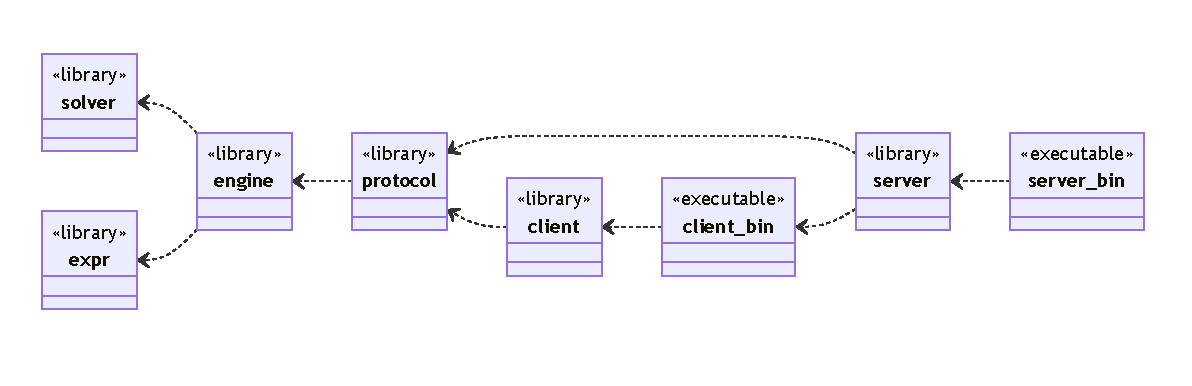
\includegraphics[width=15cm]{libsdiagram}
    \caption{Диаграмма зависимостей подпроектов\label{libsdiagramfig}}
\end{figure}

\begin{centering}
    \begin{longtable}{|l|l|l|}
        \caption{Подпроекты} \label{libstable}                                                                                                                                                 \\

        \hline \multicolumn{1}{|c|}{\textbf{Название подпроекта}} & \multicolumn{1}{c|}{\textbf{Каталог}}                                            & \multicolumn{1}{c|}{\textbf{Пункт ВКР}} \\ \hline
        \endfirsthead

        \multicolumn{3}{c}%
        {\hspace{-12.5cm}{Окончание таблицы \thetable} \vspace{1ex}}                                                                                                                           \\
        \hline \multicolumn{1}{|c|}{\textbf{Название подпроекта}} & \multicolumn{1}{c|}{\textbf{Каталог}}                                            & \multicolumn{1}{c|}{\textbf{Пункт ВКР}} \\ \hline
        \endhead

        solver                                                    & \href{https://github.com/prekel/chapgame/blob/master/lib/solver}{lib/solver}     & \ref{solverimpl}                        \\ \hline
        expr                                                      & \href{https://github.com/prekel/chapgame/blob/master/lib/expr}{lib/expr}         & \ref{expr}                              \\ \hline
        engine                                                    & \href{https://github.com/prekel/chapgame/blob/master/lib/engine}{lib/engine}     & \ref{engine}                            \\ \hline
        client                                                    & \href{https://github.com/prekel/chapgame/blob/master/lib/client}{lib/client}     & \multirow{2}{*}{\ref{clientimpl}}       \\*
        client\_bin                                               & \href{https://github.com/prekel/chapgame/blob/master/bin/client}{bin/client}     &                                         \\ \hline
        protocol                                                  & \href{https://github.com/prekel/chapgame/blob/master/lib/protocol}{lib/protocol} & \multirow{3}{*}{\ref{serverimpl}}       \\ \cline{1-2}
        server                                                    & \href{https://github.com/prekel/chapgame/blob/master/lib/server}{lib/server}     &                                         \\*
        server\_bin                                               & \href{https://github.com/prekel/chapgame/blob/master/bin/server}{bin/server}     &                                         \\ \hline
    \end{longtable}
\end{centering}

При использовании функторов, был использован <<трюк \_intf>>, который позволил вывести сигнатуру выходного модуля
в отдельный файл, что позволяет не дублировать её и в файле, где функтор реализован~\cite{intftrick}.
Т.е. в таблицах~\ref{solvermodulestable}~и~\ref{exprtable} сигнатуры выведены в файл заканчивающийся на <<\_intf.ml>>.
Там, где функторы не используются (таблица~\ref{enginemodules}), файл сигнатур имеет суффикс~<<.mli>>.

На рисунках~\ref{solvermodules} и~\ref{exprdiagramfig} представлены диаграммы с функторами,
ромбовидная стрелка из \(F\) в \(S\) означает, что функтор \(F\) параметризируется модулем, имеющим сигнатуру \(S\);
треугольная стрелка из \(F\) в \(S\) означает, что функтор \(F\) возвращает модуль с сигнатурой \(S\).
Так как функторы можно назвать параметризированными модулями, далее функторы будут называться модулями.

\section{Реализация метода решения алгебраических уравнений}\label{solverimpl}

Диаграмма модулей приведена на рисунке~\ref{solvermodules}. В таблице~\ref{solvermodulestable} показано их место в реализации и расшифровка.

\begin{figure}[H]
    \centering
    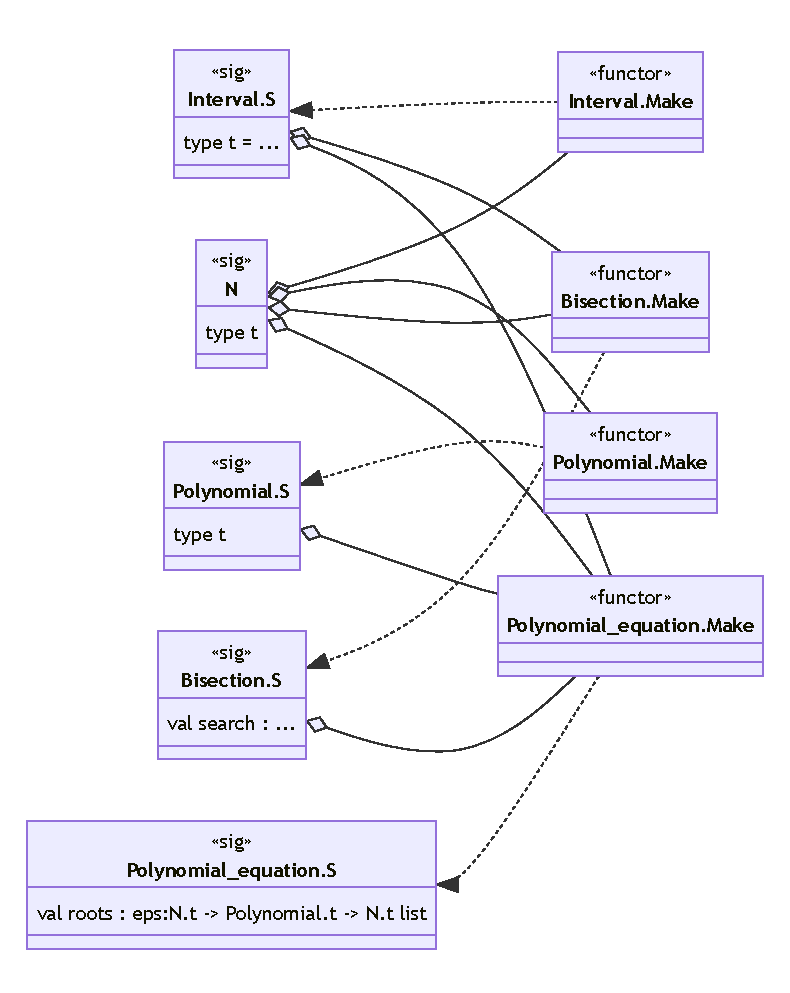
\includegraphics[width=10cm]{solver}
    \caption{Диаграмма модулей решателя алгебраических уравнений\label{solvermodules}}
\end{figure}

\begin{centering}
    \begin{longtable}{|l|l|l|}
        \caption{Модули решателя алгебраических уравнений} \label{solvermodulestable}                                                                                                                                                                                              \\

        \hline \multicolumn{1}{|c|}{\textbf{Название модуля}} & \multicolumn{1}{c|}{\textbf{Файлы}}                                                                                                      & \multicolumn{1}{c|}{\textbf{Расшифровка}}                               \\ \hline
        \endfirsthead

        \multicolumn{3}{c}%
        {\hspace{-12.5cm}{Окончание таблицы \thetable} \vspace{1ex}}                                                                                                                                                                                                               \\
        \hline \multicolumn{1}{|c|}{\textbf{Название модуля}} & \multicolumn{1}{c|}{\textbf{Файлы}}                                                                                                      & \multicolumn{1}{c|}{\textbf{Расшифровка}}                               \\ \hline
        \endhead

        \multirow{2}{*}{Interval}                             & \href{https://github.com/prekel/chapgame/blob/master/lib/solver/interval.ml}{lib/solver/interval.ml}                                     & \multirow{2}{*}{\hyperref[intervaldescr]{Промежуток}}                   \\*
                                                              & \href{https://github.com/prekel/chapgame/blob/master/lib/solver/interval\_intf.ml}{lib/solver/interval\_intf.ml}                         &                                                                         \\ \hline
        \multirow{2}{*}{Polynomial}                           & \href{https://github.com/prekel/chapgame/blob/master/lib/solver/polynomial.ml}{lib/solver/polynomial.ml}                                 & \multirow{2}{*}{\hyperref[polynomialdescr]{Многочлен}}                  \\*
                                                              & \href{https://github.com/prekel/chapgame/blob/master/lib/solver/polynomial\_intf.ml}{lib/solver/polynomial\_intf.ml}                     &                                                                         \\ \hline
        \multirow{2}{*}{Bisection}                            & \href{https://github.com/prekel/chapgame/blob/master/lib/solver/bisection.ml}{lib/solver/bisection.ml}                                   & \multirow{2}{*}{\hyperref[bisectiondescr]{Метод бисекции}}              \\*
                                                              & \href{https://github.com/prekel/chapgame/blob/master/lib/solver/bisection\_intf.ml}{lib/solver/bisection\_intf.ml}                       &                                                                         \\ \hline
        \multirow{2}{*}{Polynomial\_equation}                 & \href{https://github.com/prekel/chapgame/blob/master/lib/solver/polynomial\_equation.ml}{lib/solver/polynomial\_equation.ml}             & \multirow{2}{3.4cm}{\hyperref[equationdescr]{Алгебраическое уравнение}} \\*
                                                              & \href{https://github.com/prekel/chapgame/blob/master/lib/solver/polynomial\_equation\_intf.ml}{lib/solver/polynomial\_equation\_intf.ml} &                                                                         \\ \hline
    \end{longtable}
\end{centering}

\textbf{Промежуток}.\phantomsection\label{intervaldescr} Промежуток представлен алгебраическим типом данных
(алгебраический тип данных в функциональном программировании~-- размеченное объединение
других типов \cite{fprog-adt}),
у которого есть несколько конструкторов:

\begin{itemize}
    \item от одного вещественного числа до другого;
    \item от \(-\infty\) до заданного вещественного числа;
    \item от заданного вещественного числа до \(+\infty\);
    \item от \(-\infty\) до \(+\infty\) (вся числовая прямая);
    \item пустой промежуток.
\end{itemize}

Так же в этом модуле представлены функции для конвертации в кортеж, создания промежутка,
разбиения списка значений на промежутки, вычисления разности между правым и левым значением.

\textbf{Многочлен}.\phantomsection\label{polynomialdescr}
Многочлен представлен иммутабельным словарём, ключом которого является целое число (представляющее степень одночлена),
значением является вещественное число (представляющее коэффициент одночлена).
Предоставляет функции для создания многочлена из списка кортежей, для вычисления производной многочлена, для вычисления степени многочлена.
На рисунке~\ref{derivativecode} представлена для примера реализация функции вычисления производной многочлена. Её можно прочитать так:
<<Пары ключ-значения из словаря, которым представлен многочлен, фильтруются так, чтобы остались только с ненулевой степенью,
и заодно коэффициент преобразовывается в коэффициент производной, умножаясь на степень; далее все ключи отображаются так, чтобы стали на единицу меньше
(при этом степень не может стать отрицательной, потому что многочлен нельзя создать с отрицательной степенью у одночлена,
а на предыдущем шаге мы исключили одночлен с нулевой степенью)>>.

\begin{figure}[H]
    \centering
    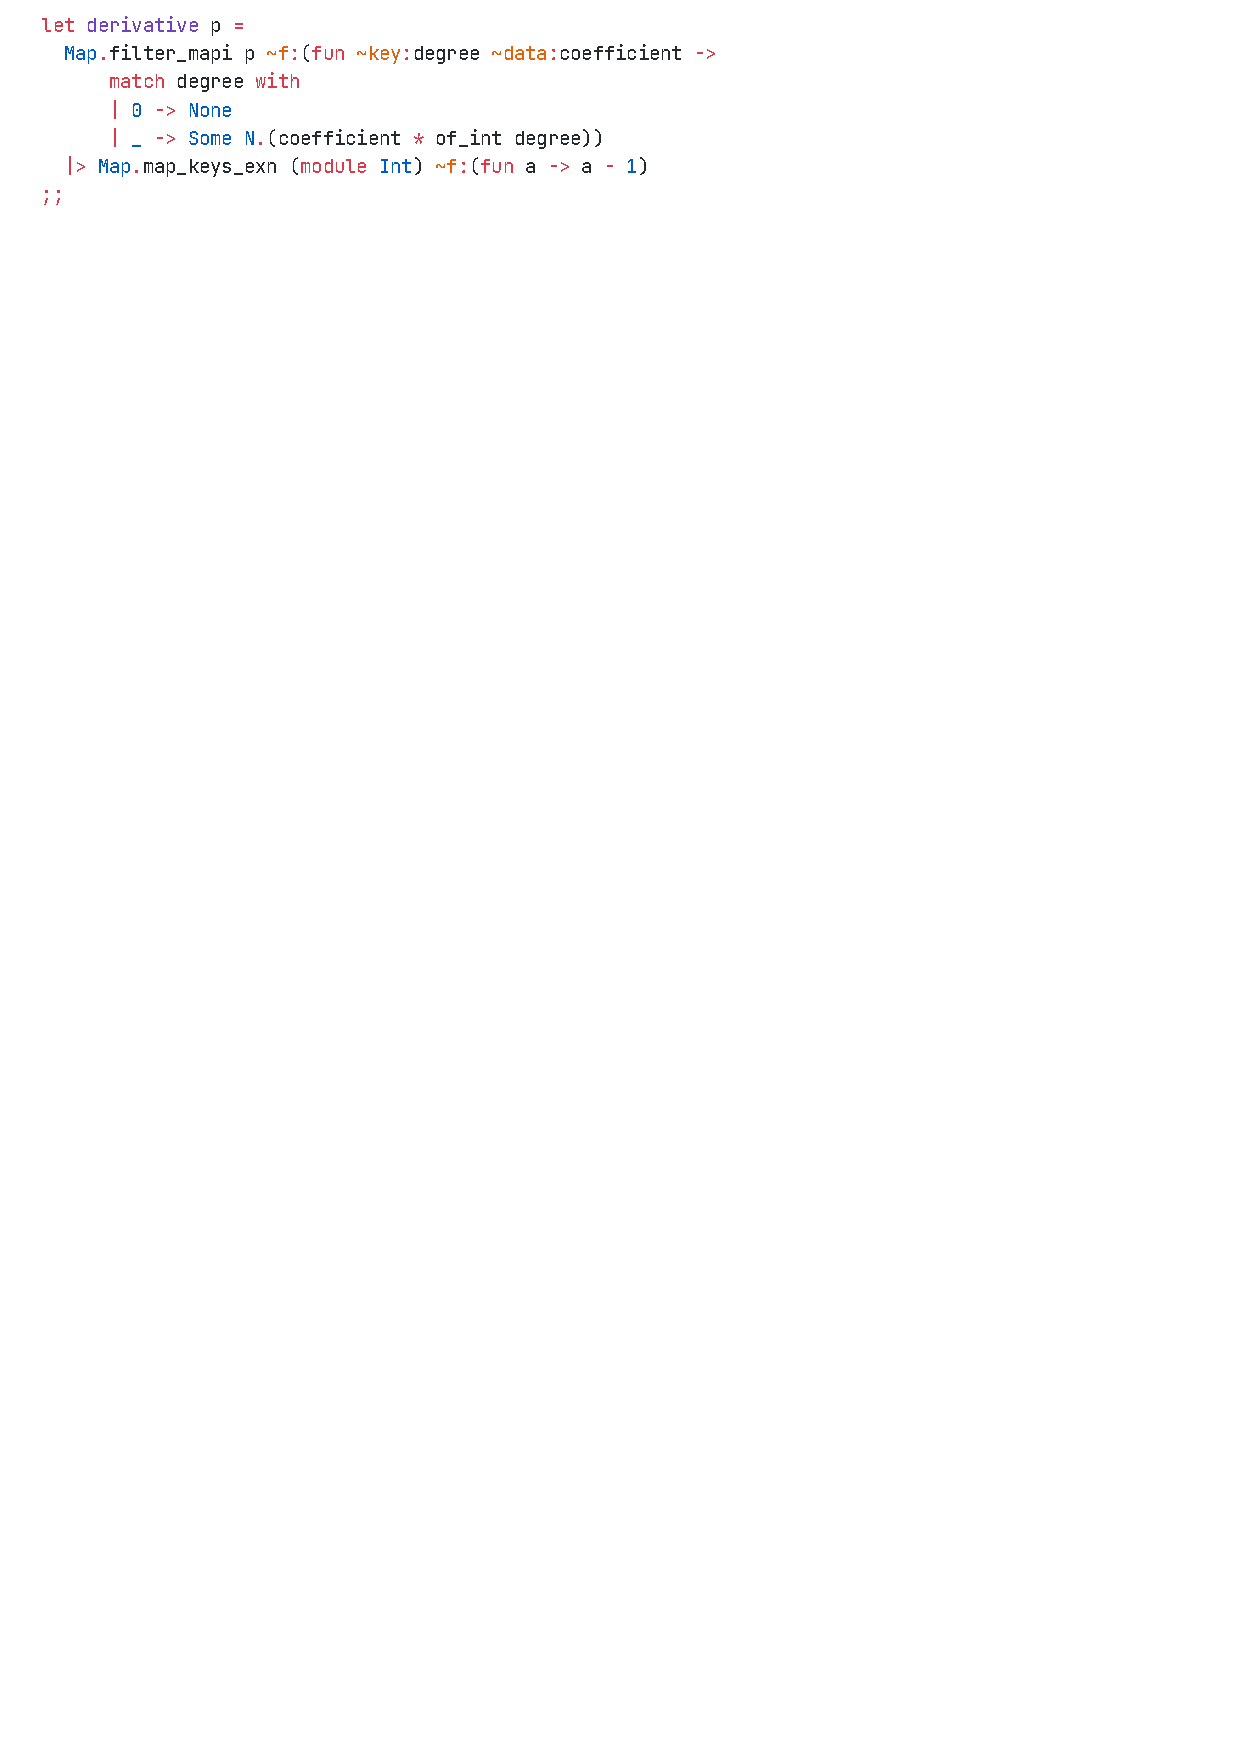
\includegraphics[width=12cm]{derivative}
    \caption{Реализация функции нахождения производной многочлена\label{derivativecode}}
\end{figure}

\textbf{Метод бисекции}.\phantomsection\label{bisectiondescr}
Этот модуль представляет функцию, принимающую другую функцию \(f(x)\), точность \(\varepsilon\)
и промежуток, на котором надо искать такой \(x\), что \(\left|f(x)\right| < \varepsilon\). Предполагается, что
функция монотонно возрастает или убывает на требуемом промежутке. Кроме самого метода бисекции, в ней реализован алгоритм,
позволяющий находить значения на бесконечном и полубесконечном промежутке, который описан в пункте~\ref{bisection}.

\textbf{Алгебраическое уравнение}.\phantomsection\label{equationdescr}
Этот модуль, используя все 3 вышеописанных, предоставляет главную функцию~-- принимающую
точность вычислений \(\varepsilon\) и многочлен \(P(x)\), и возвращающую список таких \(x\), что \(\left|P(x)\right| < \varepsilon\).
Иными словами, решает алгебраическое уравнение заданное многочленом с заданной точностью. На рисунке~\ref{rootscode}
представлена её реализация, её можно прочитать следующим образом:
<<Вычисляется степень многочлена.
Если она нулевая или отрицательная, то вернуть пустой список.
Если равна единице, решить как линейное уравнение и преобразовать в список.
Если равна двум, решить как квадратное уравнение, учитывая точность.
Иначе, вычислить производную многочлена и найти её корни; разбить список корней на промежутки и методом бисекции найти корни на промежутках>>.

\begin{figure}[H]
    \centering
    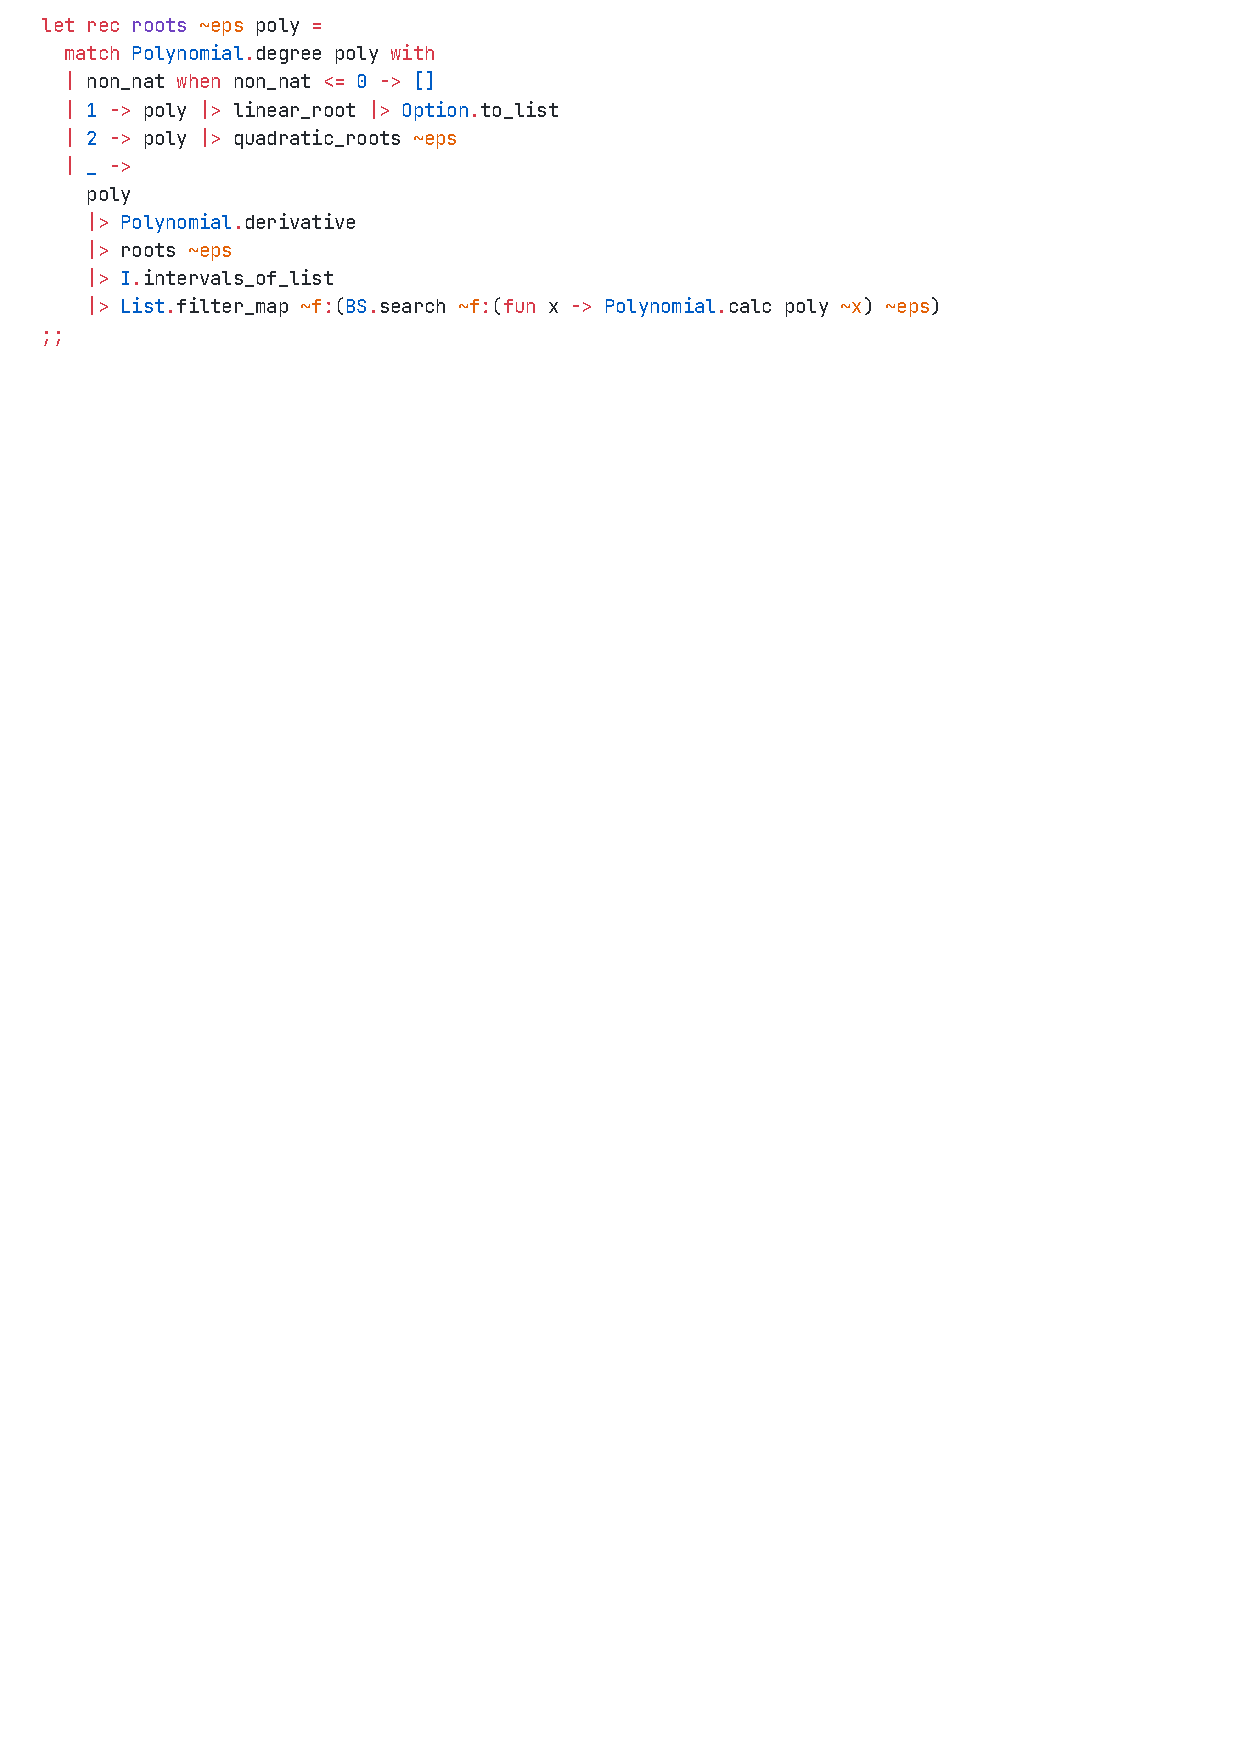
\includegraphics[width=14cm]{roots}
    \caption{Реализация функции нахождения корней алгебраического уравнения\label{rootscode}}
\end{figure}

Таким образом, реализован метод численного решения алгебраических уравнений, описанный в пункте~\ref{solvefourthdegree}.

\section{Символьные вычисления}\label{expr}

Это часть проекта призвана обобщить вычисление коэффициентов одночленов, когда требуется перемножать или складывать многочлены.
Выражения можно строить из других выражений, вычислять значения подставляя значения на место переменных в подвыражениях.
Выражения-многочлены можно складывать и перемножать, а так же вычисляя значения коэффициентов, приводить в вид многочлена,
на основе которого решается алгебраическое уравнение.
Диаграмма модулей приведена на рисунке~\ref{exprdiagramfig}. В таблице~\ref{exprtable} показано их место в реализации и расшифровка.

\begin{figure}[H]
    \centering
    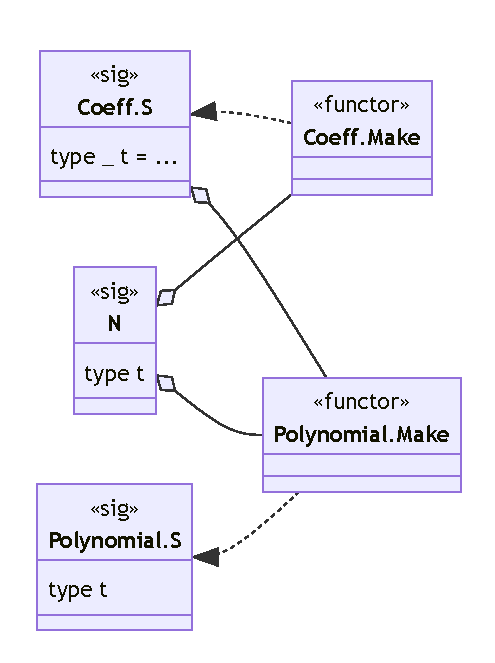
\includegraphics[width=8cm]{exprdiagram}
    \caption{Диаграмма модулей библиотеки символьных вычислений\label{exprdiagramfig}}
\end{figure}

\begin{centering}
    \begin{longtable}{|l|l|l|}
        \caption{Модули библиотеки символьных вычислений} \label{exprtable}                                                                                                                                                                       \\

        \hline \multicolumn{1}{|c|}{\textbf{Название модуля}} & \multicolumn{1}{c|}{\textbf{Файлы}}                                                                              & \multicolumn{1}{c|}{\textbf{Расшифровка}}                      \\ \hline
        \endfirsthead

        \multicolumn{3}{c}%
        {\hspace{-12.5cm}{Окончание таблицы \thetable} \vspace{1ex}}                                                                                                                                                                              \\
        \hline \multicolumn{1}{|c|}{\textbf{Название модуля}} & \multicolumn{1}{c|}{\textbf{Файлы}}                                                                              & \multicolumn{1}{c|}{\textbf{Расшифровка}}                      \\ \hline
        \endhead

        \multirow{2}{*}{Coeff}                                & \href{https://github.com/prekel/chapgame/blob/master/lib/expr/coeff.ml}{lib/expr/coeff.ml}                       & \multirow{2}{*}{\hyperref[exprdescr]{Выражение}}               \\*
                                                              & \href{https://github.com/prekel/chapgame/blob/master/lib/expr/coeff\_intf.ml}{lib/expr/coeff\_intf.ml}           &                                                                \\ \hline
        \multirow{2}{*}{Polynomial}                           & \href{https://github.com/prekel/chapgame/blob/master/lib/expr/polynomial.ml}{lib/expr/polynomial.ml}             & \multirow{2}{*}{\hyperref[exprpolydescr]{Выражение-многочлен}} \\*
                                                              & \href{https://github.com/prekel/chapgame/blob/master/lib/expr/polynomial\_intf.ml}{lib/expr/polynomial\_intf.ml} &                                                                \\ \hline
    \end{longtable}
\end{centering}

\textbf{Выражение}.\phantomsection\label{exprdescr}
Представлено обобщённым алгебраическим типом данным (GADT), так как для вычисления уравнений требуется
оперировать и скалярными, и векторными величинами. GADT позволяют построить тип так, чтобы статически разграничить выражения,
результатом вычисления которых являются скалярные или векторные величины~\cite{rwo-gadt}. При этом, для построения выражений, скалярные выражения
могут использовать векторные, и наоборот, в зависимости от операции. Например, операция, получающая проекцию вектора на ось \(X\) (<<XOfVector>>),
принимает векторное выражение и возвращает скалярное; а операция для получения вектора из его проекций, получает обе его проекции в виде скалярных выражений
и возвращает векторное выражение (рисунок~\ref{exprgadtcode}). Такая структура является деревом, а его листья это либо константы, либо
переменные, идентифицируемые отдельным типом. При этом если и полиморфные операции, такие как сумма или унарный минус, возвращающие выражение
такого же типа, что и принимают. Кроме того, есть операция <<Scope>>, позволяющая как-бы <<навесить>> нижний индекс на все переменные,
и при вычислении значения переменной, потребуется так же указать этот индекс, помимо имени переменной и её значения.

\begin{figure}[H]
    \centering
    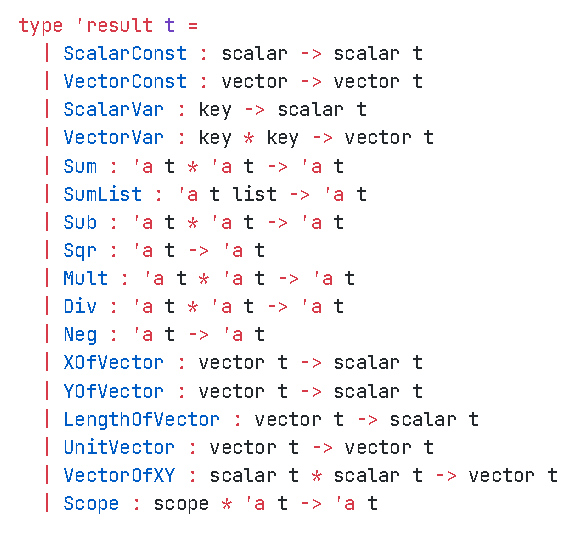
\includegraphics[width=10cm]{exprgadt}
    \caption{Определение типа выражения\label{exprgadtcode}}
\end{figure}

Чтобы не строить выражения напрямую из конструкторов, были определены отдельные функции, в том числе инфиксные операторы для операций сложения, вычитания и т.д.,
что позволило записывать выражения в привычном виде. На рисунке~\ref{exprtestfig} представлен юнит-тест, в котором строится выражение~(\ref{samleexpr}) и вычисляется
его значение при \(x = 24\) и \(y = 4\).

\begin{equation}\label{samleexpr}
    \frac{xy - x + 8}{y^2}
\end{equation}

\vspace{-2em}

\begin{figure}[H]
    \centering
    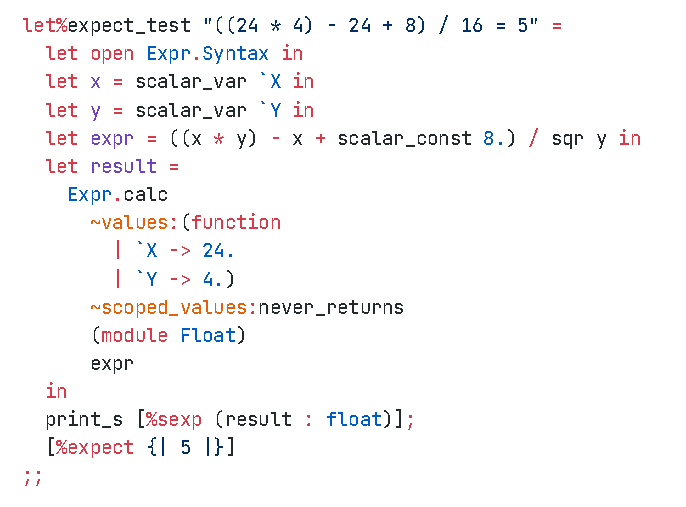
\includegraphics[width=10cm]{exprtest}
    \caption{Реализация юнит-теста для выражения\label{exprtestfig}}
\end{figure}

\textbf{Выражение-многочлен}.\phantomsection\label{exprpolydescr}
Этот модуль представляет одноместный многочлен, коэффициентами которого
являются выражения, описанные ранее. Для представления используется иммутабельный словарь, ключами которого являются целые числа~-- степень одночлена,
значения~-- выражения, описывающие коэффициенты этого одночлена. Пример использования: на рисунке~\ref{exprpolytestcode} представлен юнит-тест, в котором строится
многочлен~(\ref{samplepolyexpr}) и подставляются \(x = 24\) и \(y = 4\).

\begin{align}\label{samplepolyexpr}
    P_1(t) & = (-x + y)t^2 + (x \cdot (-y))t \nonumber           \\
    P_2(t) & = (x - y)t^2 + (x \cdot (-y))t + (-x + y) \nonumber \\
    P_1(t) & P_2(t) - P_1(t) + P_2(t)
\end{align}

\begin{figure}[H]
    \centering
    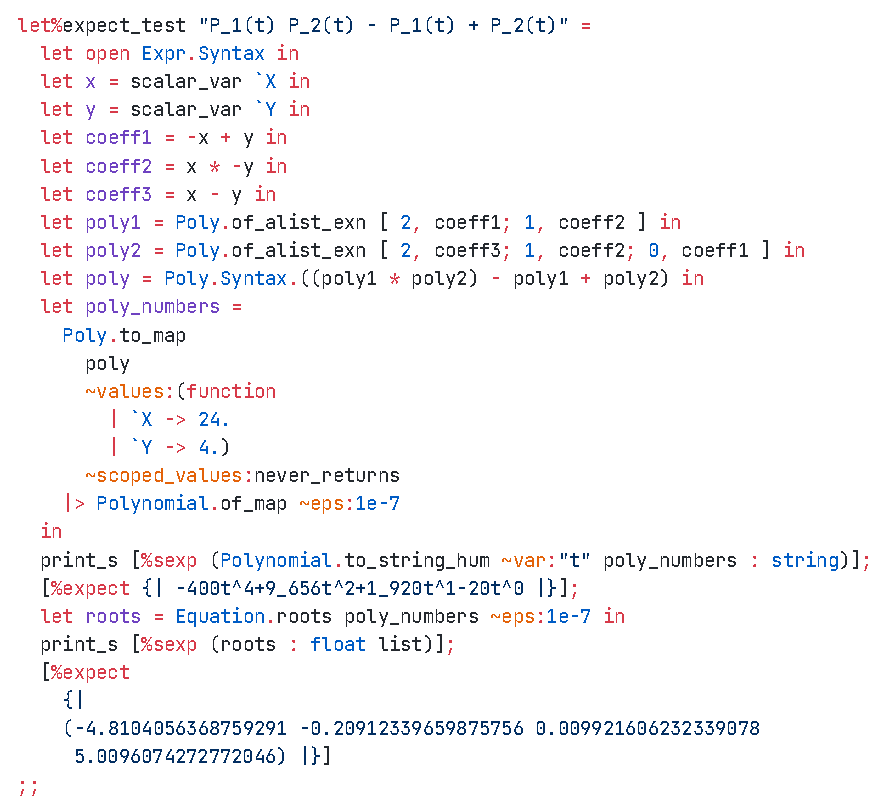
\includegraphics[width=10cm]{exprpolytest}
    \caption{Реализация юнит-теста в котором строится многочлен~(\ref{samplepolyexpr})\label{exprpolytestcode}}
\end{figure}

Из рисунка~\ref{exprpolytestcode} видно, что получен многочлен~(\ref{resultsamplepoly}) и его корни это \(x~\approx~-4.8104, x~\approx~-0.2091, x~\approx~0.0099, x~\approx~5.0096\).

\begin{equation}\label{resultsamplepoly}
    -400t^4 + 9656t^2 + 1920t - 20
\end{equation}

На рисунке~\ref{samplepolyplotfig} представлен график соответствующего уравнения, где видно примерное расположение корней.

\begin{figure}[H]
    \centering
    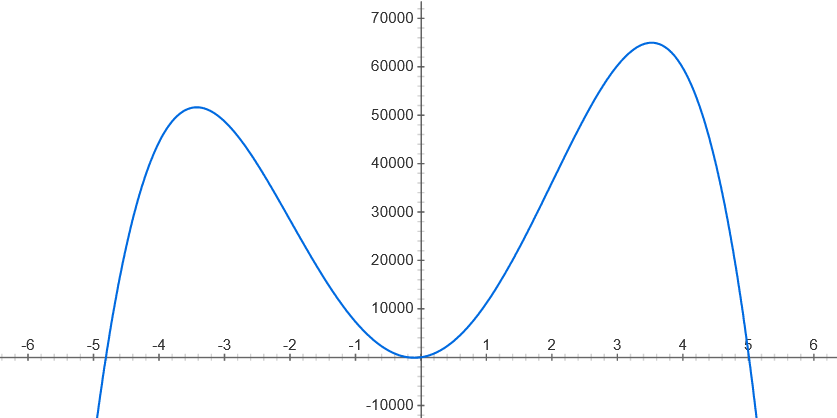
\includegraphics[width=13cm]{samplepolyplot}
    \caption{График многочлена~(\ref{resultsamplepoly})\label{samplepolyplotfig}}
\end{figure}

\section{Движок}\label{engine}

Архитектура движка имеет более плоскую и последовательную структуру, поэтому нет смысла приводить диаграмму.
В таблице~\ref{enginemodules} представлены названия модулей и файлы модулей, далее описана их работа.

\begin{centering}
    \begin{longtable}{|l|l|l|}
        \caption{Модули движка} \label{enginemodules}                                                                                                                                                                                                                            \\

        \hline \multicolumn{1}{|c|}{\textbf{Название модуля}} & \multicolumn{1}{c|}{\textbf{Файлы}}                                                                                            & \multicolumn{1}{c|}{\textbf{Расшифровка}}                                       \\ \hline
        \endfirsthead

        \multicolumn{3}{c}%
        {\hspace{-12.5cm}{Окончание таблицы \thetable} \vspace{1ex}}                                                                                                                                                                                                             \\
        \hline \multicolumn{1}{|c|}{\textbf{Название модуля}} & \multicolumn{1}{c|}{\textbf{Файлы}}                                                                                            & \multicolumn{1}{c|}{\textbf{Расшифровка}}                                       \\ \hline
        \endhead

        \hline
        \endfoot

        \multirow{2}{*}{Point}                                & \href{https://github.com/prekel/chapgame/blob/master/lib/engine/point.ml}{lib/engine/point.ml}                                 & \multirow{2}{*}{\hyperref[pointlinedescr]{Точка}}                               \\*
                                                              & \href{https://github.com/prekel/chapgame/blob/master/lib/engine/point.mli}{lib/engine/point.mli}                               &                                                                                 \\ \hline
        \multirow{2}{*}{Line}                                 & \href{https://github.com/prekel/chapgame/blob/master/lib/engine/line.ml}{lib/engine/line.ml}                                   & \multirow{2}{*}{\hyperref[pointlinedescr]{Линия}}                               \\*
                                                              & \href{https://github.com/prekel/chapgame/blob/master/lib/engine/line.mli}{lib/engine/line.mli}                                 &                                                                                 \\ \hline
        \multirow{2}{*}{Values}                               & \href{https://github.com/prekel/chapgame/blob/master/lib/engine/values.ml}{lib/engine/values.ml}                               & \multirow{2}{*}{\hyperref[valuesdescr]{Значения}}                               \\*
                                                              & \href{https://github.com/prekel/chapgame/blob/master/lib/engine/values.mli}{lib/engine/values.mli}                             &                                                                                 \\ \hline
        \multirow{2}{*}{Rule}                                 & \href{https://github.com/prekel/chapgame/blob/master/lib/engine/rule.ml}{lib/engine/rule.ml}                                   & \multirow{2}{*}{\hyperref[rulesdescr]{Правило}}                                 \\*
                                                              & \href{https://github.com/prekel/chapgame/blob/master/lib/engine/rule.mli}{lib/engine/rule.mli}                                 &                                                                                 \\ \hline
        \multirow{2}{*}{Body}                                 & \href{https://github.com/prekel/chapgame/blob/master/lib/engine/body.ml}{lib/engine/body.ml}                                   & \multirow{2}{*}{\hyperref[bodydescr]{Тело}}                                     \\*
                                                              & \href{https://github.com/prekel/chapgame/blob/master/lib/engine/body.mli}{lib/engine/body.mli}                                 &                                                                                 \\ \hline
        \multirow{2}{*}{Bodies}                               & \href{https://github.com/prekel/chapgame/blob/master/lib/engine/bodies.ml}{lib/engine/bodies.ml}                               & \multirow{2}{*}{\hyperref[bodydescr]{Тела}}                                     \\*
                                                              & \href{https://github.com/prekel/chapgame/blob/master/lib/engine/bodies.mli}{lib/engine/bodies.mli}                             &                                                                                 \\ \hline
        \multirow{2}{*}{Collision\_detection}                 & \href{https://github.com/prekel/chapgame/blob/master/lib/engine/collision\_detection.ml}{lib/engine/collision\_detection.ml}   & \multirow{2}{2cm}{\hyperref[collisiondetectiondescr]{Обнаружение столкновений}} \\*
                                                              & \href{https://github.com/prekel/chapgame/blob/master/lib/engine/collision\_detection.mli}{lib/engine/collision\_detection.mli} &                                                                                 \\ \hline
        \multirow{2}{*}{Collision\_handle}                    & \href{https://github.com/prekel/chapgame/blob/master/lib/engine/collision\_handle.ml}{lib/engine/collision\_handle.ml}         & \multirow{2}{*}{\hyperref[collisionhandledescr]{Обработка ударов}}              \\*
                                                              & \href{https://github.com/prekel/chapgame/blob/master/lib/engine/collision\_handle.mli}{lib/engine/collision\_handle.mli}       &                                                                                 \\ \hline
        \multirow{2}{*}{Action}                               & \href{https://github.com/prekel/chapgame/blob/master/lib/engine/action.ml}{lib/engine/action.ml}                               & \multirow{2}{*}{\hyperref[actiondescr]{Действие}}                               \\*
                                                              & \href{https://github.com/prekel/chapgame/blob/master/lib/engine/action.mli}{lib/engine/action.mli}                             &                                                                                 \\ \hline
        \multirow{2}{*}{Scene}                                & \href{https://github.com/prekel/chapgame/blob/master/lib/engine/scene.ml}{lib/engine/scene.ml}                                 & \multirow{2}{*}{\hyperref[scenedescr]{Сцена}}                                   \\*
                                                              & \href{https://github.com/prekel/chapgame/blob/master/lib/engine/scene.mli}{lib/engine/scene.mli}                               &                                                                                 \\ \hline
        \multirow{2}{*}{Scenes}                               & \href{https://github.com/prekel/chapgame/blob/master/lib/engine/scenes.ml}{lib/engine/scenes.ml}                               & \multirow{2}{*}{\hyperref[scenedescr]{Сцены}}                                   \\*
                                                              & \href{https://github.com/prekel/chapgame/blob/master/lib/engine/scenes.mli}{lib/engine/scenes.mli}                             &                                                                                 \\ \hline
        \multirow{2}{*}{Model}                                & \href{https://github.com/prekel/chapgame/blob/master/lib/engine/model.ml}{lib/engine/model.ml}                                 & \multirow{2}{*}{\hyperref[modeldescr]{Модель}}                                  \\*
                                                              & \href{https://github.com/prekel/chapgame/blob/master/lib/engine/model.mli}{lib/engine/model.mli}                               &                                                                                 \\ \hline
        \multirow{2}{*}{Engine}                               & \href{https://github.com/prekel/chapgame/blob/master/lib/engine/engine.ml}{lib/engine/engine.ml}                               & \multirow{2}{*}{\hyperref[enginedescr]{Движок}}                                 \\*
                                                              & \href{https://github.com/prekel/chapgame/blob/master/lib/engine/engine.mli}{lib/engine/engine.mli}                             &                                                                                 \\ \hline
    \end{longtable}
\end{centering}

\textbf{Точка} и \textbf{Линия}.\phantomsection\label{pointlinedescr} Точка определена как через её координаты по осям \(X\) и \(Y\).
Прямая линия, несмотря на то, что в модели предложено её определять через общее уравнение прямой, представлена двумя точками, находящимися на ней.
Это позволило одновременно определить кроме прямой, ещё и отрезок и луч, но для корректного обнаружения столкновений с отрезком или лучом,
в модели должны присутствовать соответствующие точки отрезка или луча.
При этом определены функции для получения коэффициентов общего уравнения прямой по формуле~(\ref{p1p2toabc}).

\begin{align}\label{p1p2toabc}
    A & = {p_2}_y - {p_1}_y \nonumber                  \\
    B & = {p_1}_x - {p_2}_x                            \\
    C & = {p_1}_y {p_2}_x - {p_1}_x {p_2}_y  \nonumber
\end{align}

\begin{Underequation}
    \(A\),~\(B\),~\(C\)~-- коэффициенты общего уравнения прямой;

    \(p_1\)~-- первая точка прямой;

    \(p_2\)~-- вторая точка прямой.
\end{Underequation}

\textbf{Значения}.\phantomsection\label{valuesdescr}
Служит для хранения значений величин. Определены через иммутабельный словарь, ключами которого являются
идентификаторы величин, а значениями являются значения этих величин.

\textbf{Правило}.\phantomsection\label{rulesdescr}
Определяет выражения-многочлены для положения и скорости тела.
При этом учитывается временной промежуток, на которых это правило действует. Правила образуют набор правил,
которые в совокупности определяют положение и скорость тела для \(t \geqslant 0\). При этом правила определяют
ещё и набор правил, который будет использоваться далее при срабатывания этого правила.
Это сделано чтобы определить правила для случаев, когда тело не движется. Т.е. определены 2 набора правил:
тот, который отражает формулы~(\ref{v_x_1}),~(\ref{v_y_1}),~(\ref{r_x_1})~(\ref{r_y_1}),~(\ref{acceleration123});
и набор из единственного правила для случая, когда тела не движется (по формулам~(\ref{rules0_0})).
При этом правило из первого набора для случая, когда \(\Constrainttge\),
указывает на второй набор правил, как тот, который следует использовать далее.
Остальные правила указывают на тот же набор правил, в котором определены.

\begin{align}\label{rules0_0}
     & v_x(t)  = 0 \nonumber   \\
     & v_y(t)  = 0 \nonumber   \\
     & x(t)    = x_0           \\
     & y(t)    = y_0 \nonumber \\
     & t \geqslant 0 \nonumber
\end{align}

\begin{Underequation}
    \(v_x(t)\)~-- проекция вектора скорости тела \(\vec{v}(t)\) в момент времени \(t\) на ось \(X\);

    \(v_y(t)\)~-- проекция вектора скорости тела \(\vec{v}(t)\) в момент времени \(t\) на ось \(Y\);

    \(x(t)\)~-- координата положения тела по оси \(X\);

    \(y(t)\)~-- координата положения тела по оси \(Y\);

    \(x_0\)~-- координата начального положения тела по оси \(X\);

    \(y_0\)~-- координата начального положения тела по оси \(Y\);

    \(t\)~-- момент времени.
\end{Underequation}

Кроме того, в этом модуле определена функция дла вычисления скорости и положения тела в момент времени \(t\),
принимающая набор правил и набор значений, возвращающая \(x(t)\), \(y(t)\), \(v_x(t)\), \(v_y(t)\) и следующий набор правил.

\textbf{Тело} и \textbf{тела}.\phantomsection\label{bodydescr}
Тело определено его идентификатором, набором значений величин, и набором правил. Набор тел
представлен иммутабельным словарём, ключи которого~-- идентификаторы тела, значения~-- тела.
Предоставляет функцию для вычисления положения тел, принимающую набор тел и момент времени
и возвращающую новый набор тел.

\textbf{Обнаружение столкновений}.\phantomsection\label{collisiondetectiondescr}
Задача функций в этом модуле вычислять время столкновения.
Для этого, уравнения, описанные в пункте~\ref{collisiondetectioneqs}, строятся путём, описанным в пункте~\ref{expr}.
Кроме попарного перебора тел и выбора наименьшего из полученных, требуется отсеять такие найденные корни, которые
не ложатся в промежутки времени, заданные правилом. Кроме того, из-за погрешности в вычислениях тела могут чуть-чуть пересекаться и
у уравнения нахождения времени столкновения будет корень, не смотря на то, что тела скорее всего направлены в разные стороны.
Т.е. следует учесть погрешность и не пытать искать время столкновения между телами, расстояние между которыми не превышает
выбранную погрешность. В случае обнаружения столкновения с лучом или отрезком, кроме вычисления времени столкновения через уравнение,
требуется дополнительно проверить, что точна столкновения находится на этом луче или отрезка, потому что она может находиться на прямой,
на которой лежит этот отрезок или луч. Для этого необходимо, чтобы углы, образованные отрезком (лучом) и отрезком от конца отрезка
до центра тела, был острым. Например, в обоих случаях уравнение обнаружило столкновение тела с соответствующим отрезком на рисунке~\ref{dotprdfig}.
Однако правый случай не следует принимать за обнаруженное столкновения. Такой случай отличается тем, что угол в правом случае
угол \(\angle A_2 B_2 C_2\) тупой, когда в левом соответствующий угол \(\angle A_1 B_1 C_1\) острый.
Это можно проверить через скалярное произведение векторов \(\vec{BA}\) и \(\vec{BC}\): если выполняется условие~(\ref{dotprodbabc}), значит этот угол острый
и тело действительно столкнулось с отрезком. Таким же образом надо проверить и угол, образованный второй точкой отрезка
(поменяв местами точки \(A\) и \(B\) в условии) и подобным образом проверяется столкновение с лучом.

\begin{equation}\label{dotprodbabc}
    \langle \vec{BA}, \vec{BC} \rangle > 0
\end{equation}

\begin{Underequation}
    \(\vec{BA}\)~-- вектор из проверяемой точки отрезка во вторую точку отрезка;

    \(\vec{BC}\)~-- вектор из проверяемой точки отрезка в центр тела.
\end{Underequation}

\begin{figure}[H]
    \centering
    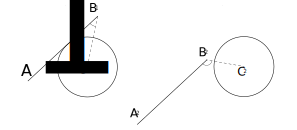
\includegraphics[width=15cm]{dotprd}
    \caption{Проверка столкновения тела с отрезком\label{dotprdfig}}
\end{figure}

\textbf{Обработка ударов}.\phantomsection\label{collisionhandledescr}
Этот модуль реализует формулы~(\ref{collisionhandle}) и~(\ref{collisionhandleafterlim}) и
предоставляет 3 функции:

\begin{itemize}
    \item для вычисления новых скоростей при столкновении двух тел;
    \item для вычисления новой скорости тела при столкновении с точной;
    \item для вычисления новой скорости тела при столкновении с прямой (лучом, отрезком).
\end{itemize}

\textbf{Действие}.\phantomsection\label{actiondescr}
Этот модуль описывает тип действия, которое можно применить к модели.
Он включает в себя время действия (т.е. время, когда это действие должно быть применено), вид действия,
параметры расчёта следующих состояний модели. Вид действия может быть одним из:

\begin{itemize}
    \item добавить тело со следующими параметрами: идентификатор, координаты положения, радиус, коэффициент трения, масса;
    \item добавить тело, присвоив ему параметры из переданного ассоциативного списка <<идентификатор переменной>>-<<значение>>;
    \item добавить точку;
    \item добавить линию (луч, отрезок);
    \item придать скорость телу, передаётся идентификатор тела и новая скорость;
    \item удалить тело по его идентификатору;
    \item удалить точку;
    \item удалить линию (луч, отрезок);
    \item обновить параметры тела по его идентификатору и ассоциативному списку значений;
    \item обновить глобальный параметр.
\end{itemize}

Параметры расчёта задаются:

\begin{itemize}
    \item промежутком времени, на которое следует просчитать состояния модели, начиная от времени совершения действия;
    \item количеством столкновений, которое следует просчитать начиная от времени совершения действия.
\end{itemize}

Оба параметра являются опциональными. Если заданы оба~-- расчёт происходит до того, который наступит быстрее.
Если не задан никакой~-- то рассчитываются все столкновения до того момента, пока тела не остановятся.
Если у какого-то тела коэффициент равен нулю, или ускорение свободного падение равно нулю, то ускорения одного или всех тел будет равно нулю.
В таком случае, тела могут не остановиться никогда: если эти тела находятся в замкнутом пространстве, то столкновения будут происходить бесконечно
и при попытке рассчитать, не указав параметры, произойдёт бесконечное зацикливание. Обработка таких ситуаций не предусмотрена и программу придётся перезапускать,
так что подбор оптимальных параметров расчёта ложится на пользователя. Однако, если тела могут продолжить двигаться и между ними не будет происходить столкновений,
такая ситуация успешно обработается, что позволит, например, вычислять число \(\pi\) методом Гальперина, что описано в пункте~\ref{pipool}.

\textbf{Сцена} и \textbf{сцены}.\phantomsection\label{scenedescr}
Этот модуль определяет сцену, а именно~-- её время, наборы тел, точек, линий, глобальные значения, и причину возникновения.
Как определён набор тел, описано ранее. Наборы точек и линий представлены иммутабельными множествами: т.е. не имеют
отдельного идентификатора и идентифицируются своим значением непосредственно. Причиной может
служить пользовательское действие, или столкновение, или инициализация.

Кроме того, в данном модуле представлен подмодуль, отвечающий за вычисление разницы между двумя сценами.
Разница вычисляется между старой и новой сценой, поэтому в разнице представлено новое время,
разница между наборами тел, разница между наборами точек, разница между наборами линий, разница глобальных значений, новая причина.
При этом разница между наборами, которые представлены словарём, представлена в виде ассоциативного списка добавленных и изменённых пар
идентификатор-значение и списка удалённых идентификаторов;
разница между наборами, которые представлены множеством, представлена в виде списка добавленных и списка удалённых значений.
Кроме функции для вычисления разницы, определена функция для применения разницы: она принимает старый набор, разницу, и возвращает новый набор.

Набор сцен представлен как иммутабельный словарь, ключами которого является время сцены, значениями~-- значение сцены.
Хранение в таком виде позволяет эффективно определить функцию, которая делает срез сцен до требуемого времени.
Эта функция понадобится далее для работы движка.

\textbf{Модель}.\phantomsection\label{modeldescr}
Модель представлена опциональным временем до которого рассчитаны сцены и набором сцен.
Это время может быть не предоставлено, когда расчёт произведён до того момента как столкновения прекратятся.
Как указано ранее, такой расчёт можно сделать, не указав параметры расчёта.
Этот модуль так же предоставляет подмодуль для вычисления разницы между моделями.

\textbf{Движок}.\phantomsection\label{enginedescr}
Кроме того, что этот модуль реализует ключевую функциональность, он является основным в библиотеке и указывает на модули, которые
должны быть доступны из других библиотек (так работает система сборки:
если в библиотеке есть файл с названием идентичным названию библиотеки, то из других библиотек будет доступен только этот модуль,
а остальные нужные модули должны быть переобъявлены в нём).

Ключевая функциональность заключена в двух функциях.
Одна позволяет: или применить действие, или применить разницу моделей,
или продлить используя заданные параметры расчёта, или заменить модель.
Кроме этого она принимает старую модель, а возвращает новую.
Вторая функция позволяет только применить действие или продлить вычисление, но кроме новой модели
возвращает разницу между старой и новой. Вторая функция используется на сервере потому
что требуется передавать подключённым клиентам разницу.
Эти функции реализованы с помощью следующих, которые не попадают в файл сигнатуры модуля движка и остаются сокрытыми.

Функция получения последовательности сцен. На основе одной сцены строится следующая,
и так по цепочке, образуя бесконечную ленивую последовательность.
Новое время сцены вычисляется с помощью описанного ранее модуля обнаружения столкновений.
Скорости тел перерассчитываются на основе описанного ранее модула обработки ударов.
Эта функция принимает опциональный временной параметр, который принуждает прекратить
последовательность на сцене с конкретным временем.

Функция применения действия к сцене. Отвечает за обработку действия.
Например если действие~-- <<добавить точку>>, то возвращается сцена с обновлённым набором точек, содержащим новую точку.

Функция применения действия к модели. Работает по следующему алгоритму:

\begin{itemize}
    \item вычисляется набор сцен до времени действия;
    \item на основе последней сцены из этого набора строится последовательность сцен до времени действия;
    \item к последней сцене из последовательности, полученной на предыдущем шаге, применяется действие;
    \item на основе полученной сцены, строится последовательность следующих сцен и из них берутся первые сцена на основе параметров расчёта;
    \item в новую модель назначается время, до которого рассчитаны сцены, и набор сцен из предыдущего шага.
\end{itemize}

Подобным образом реализована функция продления, а для вычисления разницы используется соответствующая функция из модуля модели.
Таким образом, движок можно условно считать стейт-машиной (с тем условием, что число состояний бесконечно),
где множество состояний это множество моделей, а функция перехода это вышеописанная функция применения действия к модели.

Подробнее об единицах измерения. Конкретные единицы измерения не используются.
При этом, при определении величин соблюдается консистентность: например для определения скорости используются
те же самые условные единицы времени и расстояния, что и для самих времени и расстояния. Это позволяет на деле использовать
любые единицы измерения: далее, при реализации клиентской части для единицы времени используется 1 секунда,
для единицы расстояния 1 пиксель. Для массы выбирать конкретную единицу измерения не имеет смысла, потому что во всех
использованных формулах, в которых присутствует масса, единицы измерения сокращаются.

\section{Клиентская часть}\label{clientimpl}

Как указано ранее, клиентская часть реализована в виде браузерного одностраничного приложения.
Оно может может работать независимо от серверной части: тогда будет доступен только одиночный режим,
когда все вычисления проходят на клиенте. Независимость от сервера позволяет развернуть приложение на
любом хостинге статических веб-приложений, например GitHub Pages, что и было сделано:
\underline{\smash{\href{https://prekel.github.io/chapgame/}{https://prekel.github.io/chapgame/}}}.

Клиентская часть разделена на компоненты, каждый из которых в себе инкапсулирует состояние.
Визуально приложение поделено на две части: слева располагаются заголовок,
вкладки переключения одиночного и многопользователького режима, панели управления;
а справа отрисовывается текущее состояние.
Заголовок состоит из иконки вызова справочной информации
и иконки-ссылки на репозиторий с исходным кодом. Далее перечислены панели в порядке их
расположения сверху вниз как на рисунках~\ref{screen1fig} и~\ref{screen2fig}.

\textbf{Панель состояния}. Через неё можно экспортировать или импортировать модель.
Используется текстовое представление, а именно S-выражения. Здесь же можно полностью очистить модель и
получить статистику:

\begin{itemize}
    \item количество сцен;
    \item количество причин для возникновения сцен;
    \item столкновений среди них;
    \item столкновений между телами, между телом и линией, между телом и точкой среди них;
    \item пользовательских действий;
    \item время, до которого рассчитана модель (\(\infty\), если рассчитано до того состояния, при котором не будет новых столкновений);
    \item время последней сцены.
\end{itemize}

\textbf{Панель времени}. Позволяет установить текущее время воспроизведения через текстовый ввод или кнопки,
которые отматывают на секунду назад, вперёд или в нулевой момент времени.

\textbf{Панель параметров расчёта}.
Позволяет установить параметры расчёта, описанные ранее.

\textbf{Панель скорости}. Установка скорости происходит аналогично со временем, только кнопки
позволяют уменьшить или увеличить скорость на \(0.1\), поставить единичную скорость или
отрицательную единичную скорость, или поставить воспроизведение на паузу.
При поставке воспроизведения на паузу, скорость ставиться на нулевую и меняется иконка этой кнопки;
при повторном нажатии, скорость возвращается на то значение, которое было при постановке на паузу.

\textbf{Панель тел}.
На этой панели расположена таблица с текущими параметрами тел
(идентификатор, координаты, коэффициент трения, масса, радиус, проекции вектора скорости),
вычисляемыми величинами (длина вектора скорости, проекции и длина вектора ускорения),
а так же кнопки для изменения параметров и удаления тела.
Кроме таблицы, на этой панели расположена кнопка, вызывающая модальное окно,
позволяющее создавать новые тела.

\textbf{Панель линий}. На этой панели расположена таблица линий, в ней
показано то, что и использовалось при реализации линий,
а именно координаты двух точек и вид линии (прямая линия, или луч, или отрезок).
В таблице есть кнопка для удаления линии. Добавление линии реализовано в модальном окне.
Изменять линии нельзя, можно только удалить её и добавить новую с нужными параметрами.

\textbf{Панель точек}. Аналогично с панелью линий.

\textbf{Панель глобальных параметров}. Здесь можно задать ускорение
свободного падения, от которого, по формуле~(\ref{acceleration123}), зависит ускорение тел.
Допускается использовать отрицательное значение: это не обрабатывается по особому сознательно,
но в этом случае ускорение тел станет сонаправлено их скорости.

\begin{figure}[H]
    \centering
    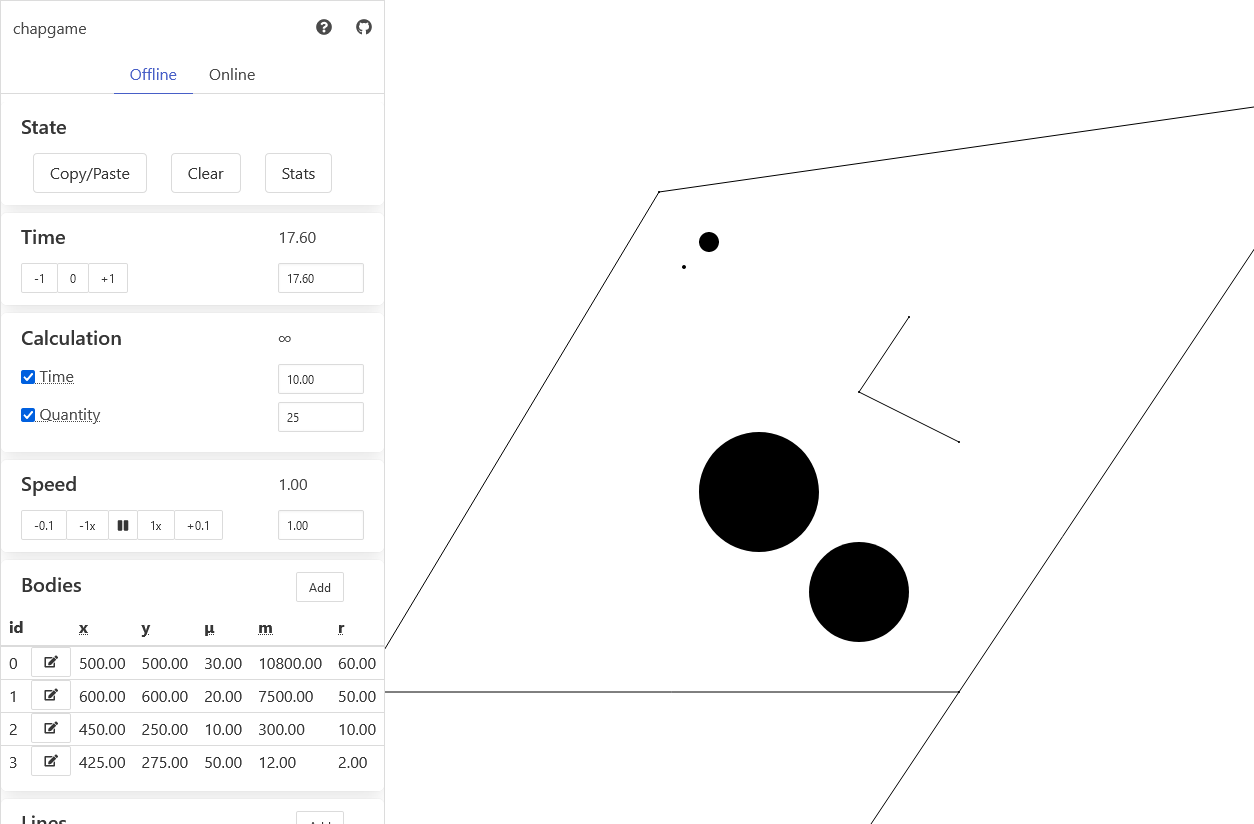
\includegraphics[width=15cm]{screen1}
    \caption{Заголовок, вкладки, панели состояния, времени, скорости, тел\label{screen1fig}}
\end{figure}

\begin{figure}[H]
    \centering
    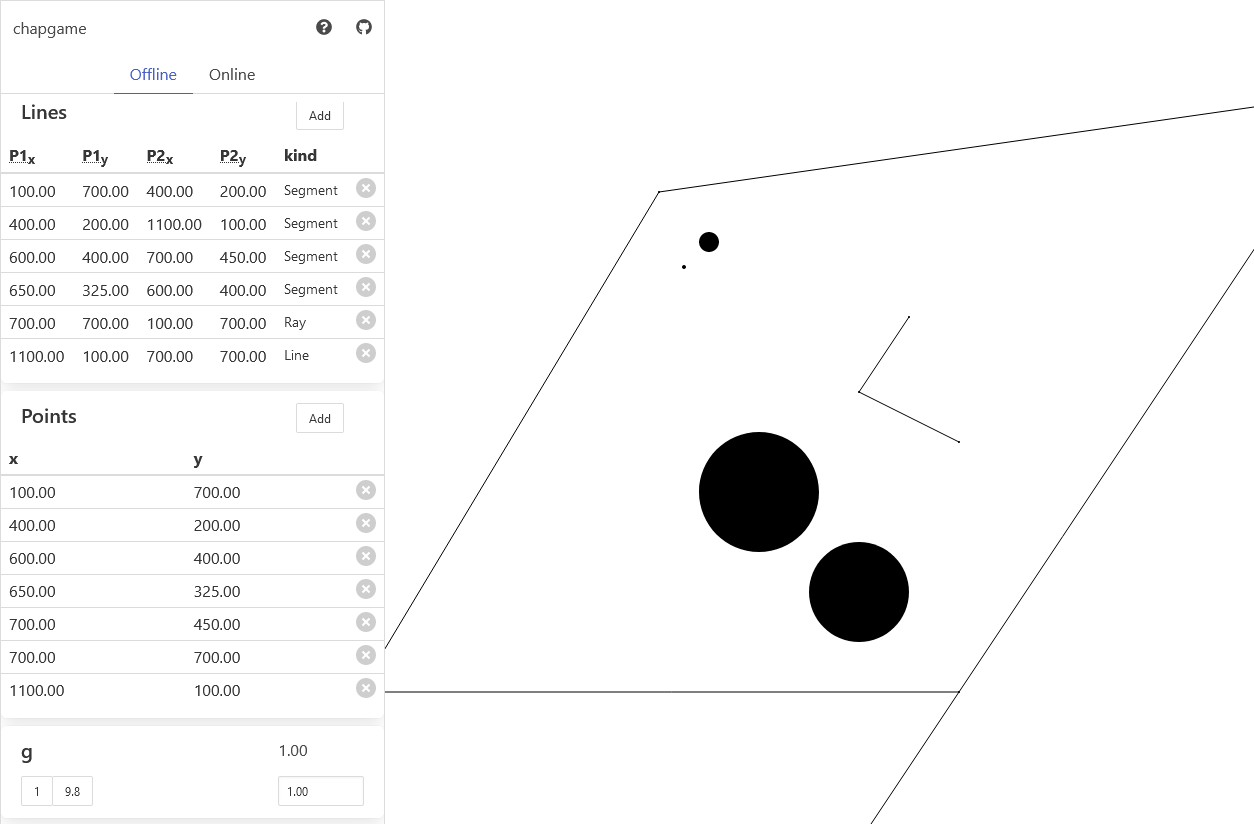
\includegraphics[width=15cm]{screen2}
    \caption{Панели линий, точек, глобальных параметров\label{screen2fig}}
\end{figure}

Сама сцена отрисовывается с помощью SVG (Scalable Vector Graphics~-- масштабируемая векторная графика).
Так как SVG можно встраивать в HTML~\cite{mdnsvgtag}, им можно манипулировать так же как и остальными элементами с помощью используемой UI-библиотеки Bonsai.
Воспроизведение происходит с частотой 60 кадров в секунду:
т.е. 60 раз в секунду текущее время увеличивается на \(\frac{s}{60}\), где \(s\)~-- скорость воспроизведения.
Сцену можно перемещать и менять масштаб. При изменении масштаба, увеличение или уменьшение происходит по направлению положения курсора.
Управление осуществляется посредством нажатия на фигуры: чем дальше от центра тела произошло нажатие, тем больше придаваемая скорость.

Так как масштаб изменяется через колесо мыши, потребовалось использовать соответствующий Web~API~\cite{mdn-wheel}.
Однако, используемый компилятор js\_of\_ocaml имел биндинги только к устаревшим API для работы с колесом мыши~\cite{jsoo-issue-1272}.
Поэтому был сделать пул-реквест в репозиторий js\_of\_ocaml под номером
\href{https://github.com/ocsigen/js\_of\_ocaml/pull/1273}{\#1273}, который предоставляет биндинги для современного API.
В последствии он был принят командой разработки и слит в основную ветку.

\section{Серверная часть}\label{serverimpl}

Задачи сервера:

\begin{itemize}
    \item API многопользовательского режима;
    \item раздача статики (HTML-файл и скомпилированный JavaScript-файл клиентской части).
\end{itemize}

API многопользовательского режима представляет REST-подобный интерфейс,
с помощью которого можно создать <<комнату>> (т.е. модель, ассоциированную с подключёнными клиентами),
послать действие, которое применится к модели на сервере, и послать запрос, который инициализирует WebSocket-соединение,
по которому будут приходить изменения (разница) модели. Кроме модели, в комнате храниться время и скорость,
изменения которых так же синхронизируются с клиентами. Для передачи данных используется формат S-выражений.

Статика встраивается статически в исполняемый файл сервера, поэтому на рисунке~\ref{libsdiagramfig} библиотека сервера зависит от клиента.

Вместе с ответом на HTTP-запрос корневого HTML-документа, сервер посылает cookie со специальным значением,
которое затем программно считывается на клиентской части, что позволяет в ней активировать дополнительную функциональность~--
многопользовательский режим. В этом режиме используется разбор адресной строки (роутинг; т.е. можно сказать,
имитируется многостраничное приложение):

\begin{itemize}
    \item <</>>~-- одиночный режим;
    \item <</online>>~-- меню создания комнаты или ввода идентификатора существующей;
    \item <</online/:id>>~-- многопользовательский режим (комната с идентификатором <<:id>>).
\end{itemize}

При создании комнаты автоматически назначается токен, который в адресную строку передаётся как query-параметр,
без которого можно только наблюдать за состоянием комнаты без права посылать действия.
